%\documentclass{beamer}
\documentclass[handout]{beamer}
\setbeamercovered{transparent}

\usepackage[utf8]{inputenc}

\usepackage[german]{babel}
\usepackage{color}
\usepackage{xcolor}
\usepackage{graphicx}
\usepackage{tikz}
\usepackage{Latex_Template/beamerthemeFOSSAG}
\usepackage{subfiles}

 


\title{SSH}
\subtitle{Kontrolle aus der Ferne}
\author{@innaytool [Yannick Bungers] \\ innay@foss-ag.de}
\institute{FOSS AG}
\date{\today}

\begin{document}

\begin{frame}
\titlepage
\end{frame}

% Dateien
%\subfile{content.tex}
\subfile{motivation.tex}
\subfile{history.tex}
\subfile{introduction.tex}
%\subfile{test.tex}
\subfile{software.tex}
%\subfile{sshsub.tex}
\subfile{sftp.tex}
\subfile{scp.tex}
\subfile{sshfs.tex}
\subfile{remoteexec.tex}
%\subfile{porttunnel.tex}
\begin{frame}
	\frametitle{SOCKS5 Proxy}
	\begin{itemize}
		\item \texttt{ssh -N -D <port> <server>} $\rightarrow$ SOCKS5 Proxy
		\item Tunnel zu einem Server für beliebige Ports
		\item Ähnlich zu einem VPN
		\item Proxy
	\end{itemize}
\end{frame}
\begin{frame}
\frametitle{Local Single Port Tunnel}
\texttt{ssh -N -L <BindAdresse>:\textit{<BindPort>}: <ZielAdresse>:\textit{<ZielPort>} <jumpServer> }

Auf dem lokalen Rechner wird der Port und die Adresse gebunden
\end{frame}

\begin{frame}
	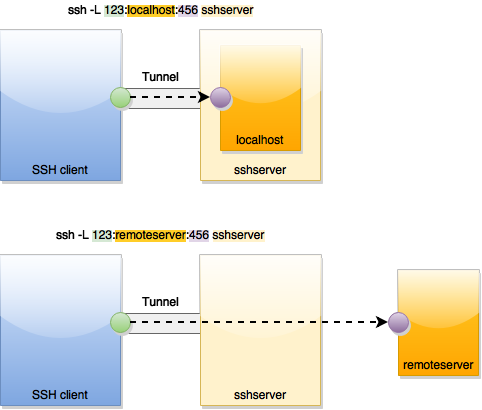
\includegraphics[scale=0.55]{ssh-L-tunnel.png}
\end{frame}

\begin{frame}
\frametitle{Remote Single Port Tunnel}
\texttt{ssh -N -R <BindAdresse>:\textit{<BindPort>}: <ZielAdresse>:\textit{<ZielPort>} <jumpServer>}\\
Auf dem entfernten Rechner wird die Addresse und der Port gebunden
\end{frame}

\begin{frame}
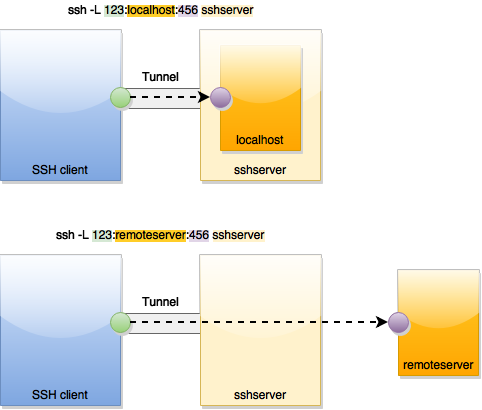
\includegraphics[scale=0.55]{ssh-L-tunnel.png}\\
\end{frame}

\subfile{server.tex}
\subfile{sshkey.tex}
\subfile{summary.tex}

\end{document}